% !TEX root = ../thesis.tex

\section{Структура симуляційного програмного забезпечення}

Програма написана   на мові C++ та умовно поділяється на дві логічні частини: модуль обробки параметрів та модуль симуляції.

Модуль обробки параметрів дозволяє задавати розмір матриць, режим одноно гравця чи двох, межі перебору стратегій розрізання, параметри планувальника, характеристики обчислювальних модулів, параметрів мережі – bandwidth та latency без перековпіляції програми через параметри командного рядка.

Модуль симуляції генерує задачі для кожного з користувачів, зливає їх в один список та власне подає їх на симулятор, який повертає оброблені задачі з проставленими змінними часу початку та завершення роботи над задачею і номером обчислювального вузла, який обробляю цю  задачу.

Етапи роботи симулятора:
\begin{itemize}
	\item[1.] Перемішування списка очікуючих задач з метою емуляцїї отримання задач у випадковому порядку.
	
	\item[2.] Сортування списка очікуючих задач по складності у відповідності до пріорітетності задач та списка обчислювальних вузлів по потужності у відповідності до пріорітетності обчилювальних вузлів. Наприклад для minmax планувальника список очікуючих задач буде відсортованим від простої до складної, а список обчислювальних вузлів від потужного до повільного.
	
	\item[3.] Ініціалізація початкових задач для обчислювальних вузлів вилучаючи перші елементи з  відсортованих списків очікуючих задач та вузлів, проставлення початкового часу, який на даний момент рівний 0, та обчислення часу очікуваного завершення виконання задачі. Структури з посиланням на задачу, обчислювальний вузол та даними про початок та завершення виконання задачі поміщаються у чергу з пріорітетом по найменшому часу завершення.
	
	\item[4.] Взяти з пріорітетної черги задачу, яка буде найближчою по часу наступною виконаною задачею. Приняти час симуляції за час завершення взятої з черги задачі, додати задачу до списку виконаних задач разом із даними про час її завершення.
	
	\item[5.] Якщо список очікуючих задач не пустий, то вилучити перший елемент, поставити час початку як час симуляції, обчислити час завершення та додати у чергу з прірітетом, поставивши обчислювальний вузол як перший вільний із відсортованого списка вузлів.
	
	\item[6.] Якщо пріорітетна черга не пуста, то повернутися на крок 4.
	
	\item[7.] Знайти у списку виконаних задач найпізніші повернені задачі для кожного з користувачів та повернути їх час завершення.
\end{itemize}

\begin{figure}[H]
	\centering
	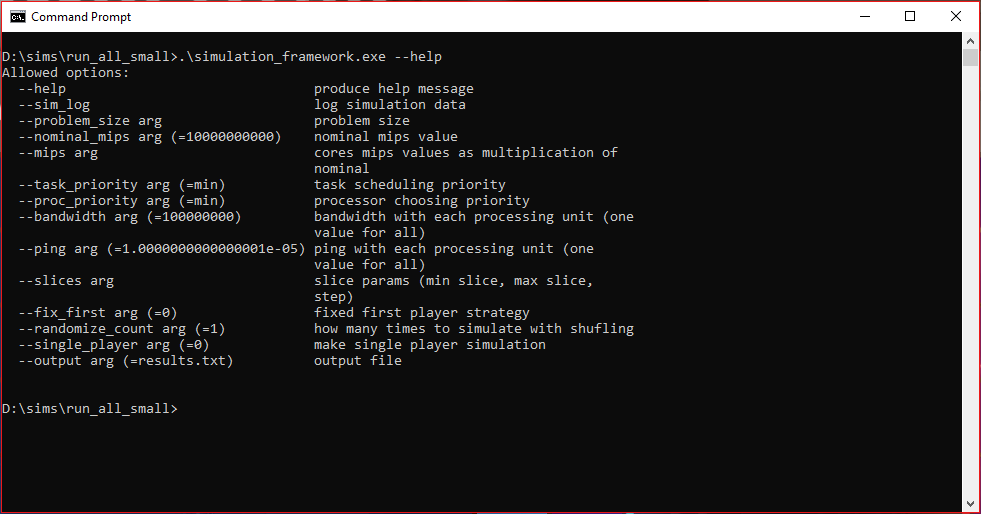
\includegraphics[width=\textwidth]{practice/img/help_ilustration}
	\caption{Скріншот вікна з описом параметрів програми}
	\label{fig:help_ilustration}
\end{figure}

На Рис. \ref{fig:help_ilustration} зображено основний інтерфейс програми. Програма має деякі обов'язкові параметри та опціональні - тобто такі, для яких вписані значення за вмовчанням, але при потребі їх можна змінити.

Список обов'язкових параметрів:
\begin{itemize}
	\item[1.] $problem\_size$ - цей параметр відповідає за визначення розміру матриць, симуляція яких буде проводитись. Розмір визначається одним числом оскільки ми матриці вважаємо квадратними - $N \times N$.
	\item[2.] $mips$ - цей параметр приймає список чисел, які визначають кількість обчислювальних вузлів у розподіленому середовищі та їх потужності. Для простоти було вирішено приймати потужності як коефіцієнти при деякій номінальній потужності, яка задається опціональним параметром $nominal\_mips$. Наприклад параметри "1 1.5 5 6" задають 4 обчислювальних вузла з потужностями $1*nominal\_mips, 1.5*nominal\_mips, 5*nominal\_mips, 6*nominal\_mips$
	\item[3.] $slices$ - параметер відповідає за вибір набору стратегій, симуляція яких буде проводитись. У випадку двох гравців це буде декартовий добуток цієї множини с собою.
\end{itemize}

Список опціональних параметрів:
\begin{itemize}
	\item[1.] $nominal\_mips$ - задає номінальний множник потужностей ОВ. За вмовченням вибраний такий, що відповідає за множення матриць розмірів 2000 за 1.6 секунди, що відносно відповідає потужності одного ядра у сучасних комп'ютерах.
	\item[2.] $bandwidth$ - регулює ширину канала для передачі даних з кожним ОВ.
	\item[3.] $ping$ - виставляє штраф за з'єднання.
	\item[4.] $single$ - булевий параметр $\{0,1\}$, який дозволяє проводити симуляції лише для одного користувача.
	\item[5.] $task\_priority$ - визначає пріорітетність вибору задач. Може приймати 2 значення - $min$ чи $max$. При виборі $min$ спочатку виконуються задачі з меншим обсягом обчислень, а для $max$ навпаки - з більшим. За вмовчуванням береться режим $min$.
	\item[6.] $proc\_priority$ - аналогічно до $task\_priority$ визначае правило вибору вільного процесора. Для $min$ задача планується на вільний процесор з найменшою потужністю, для $max$ з найбільшою.
\end{itemize}

